%\chapter{daq-comp}
\section{DAQ}
\label{sec:daq}


This section outlines the data acquisition system for ProtoDUNE.  The DAQ
system is shown in figure \ref{fig:daq-overview} along with its interfaces
to the cold electronics, and online computing systems.


\begin{cdrfigure}[DAQ Overview]{daq-overview}{Detailed overview of the DAQ system, its interconnections, data flow, timing and control signals, and the interfaces to the electronics and online computing systems \fixme{simplify diagram for TDR}}
        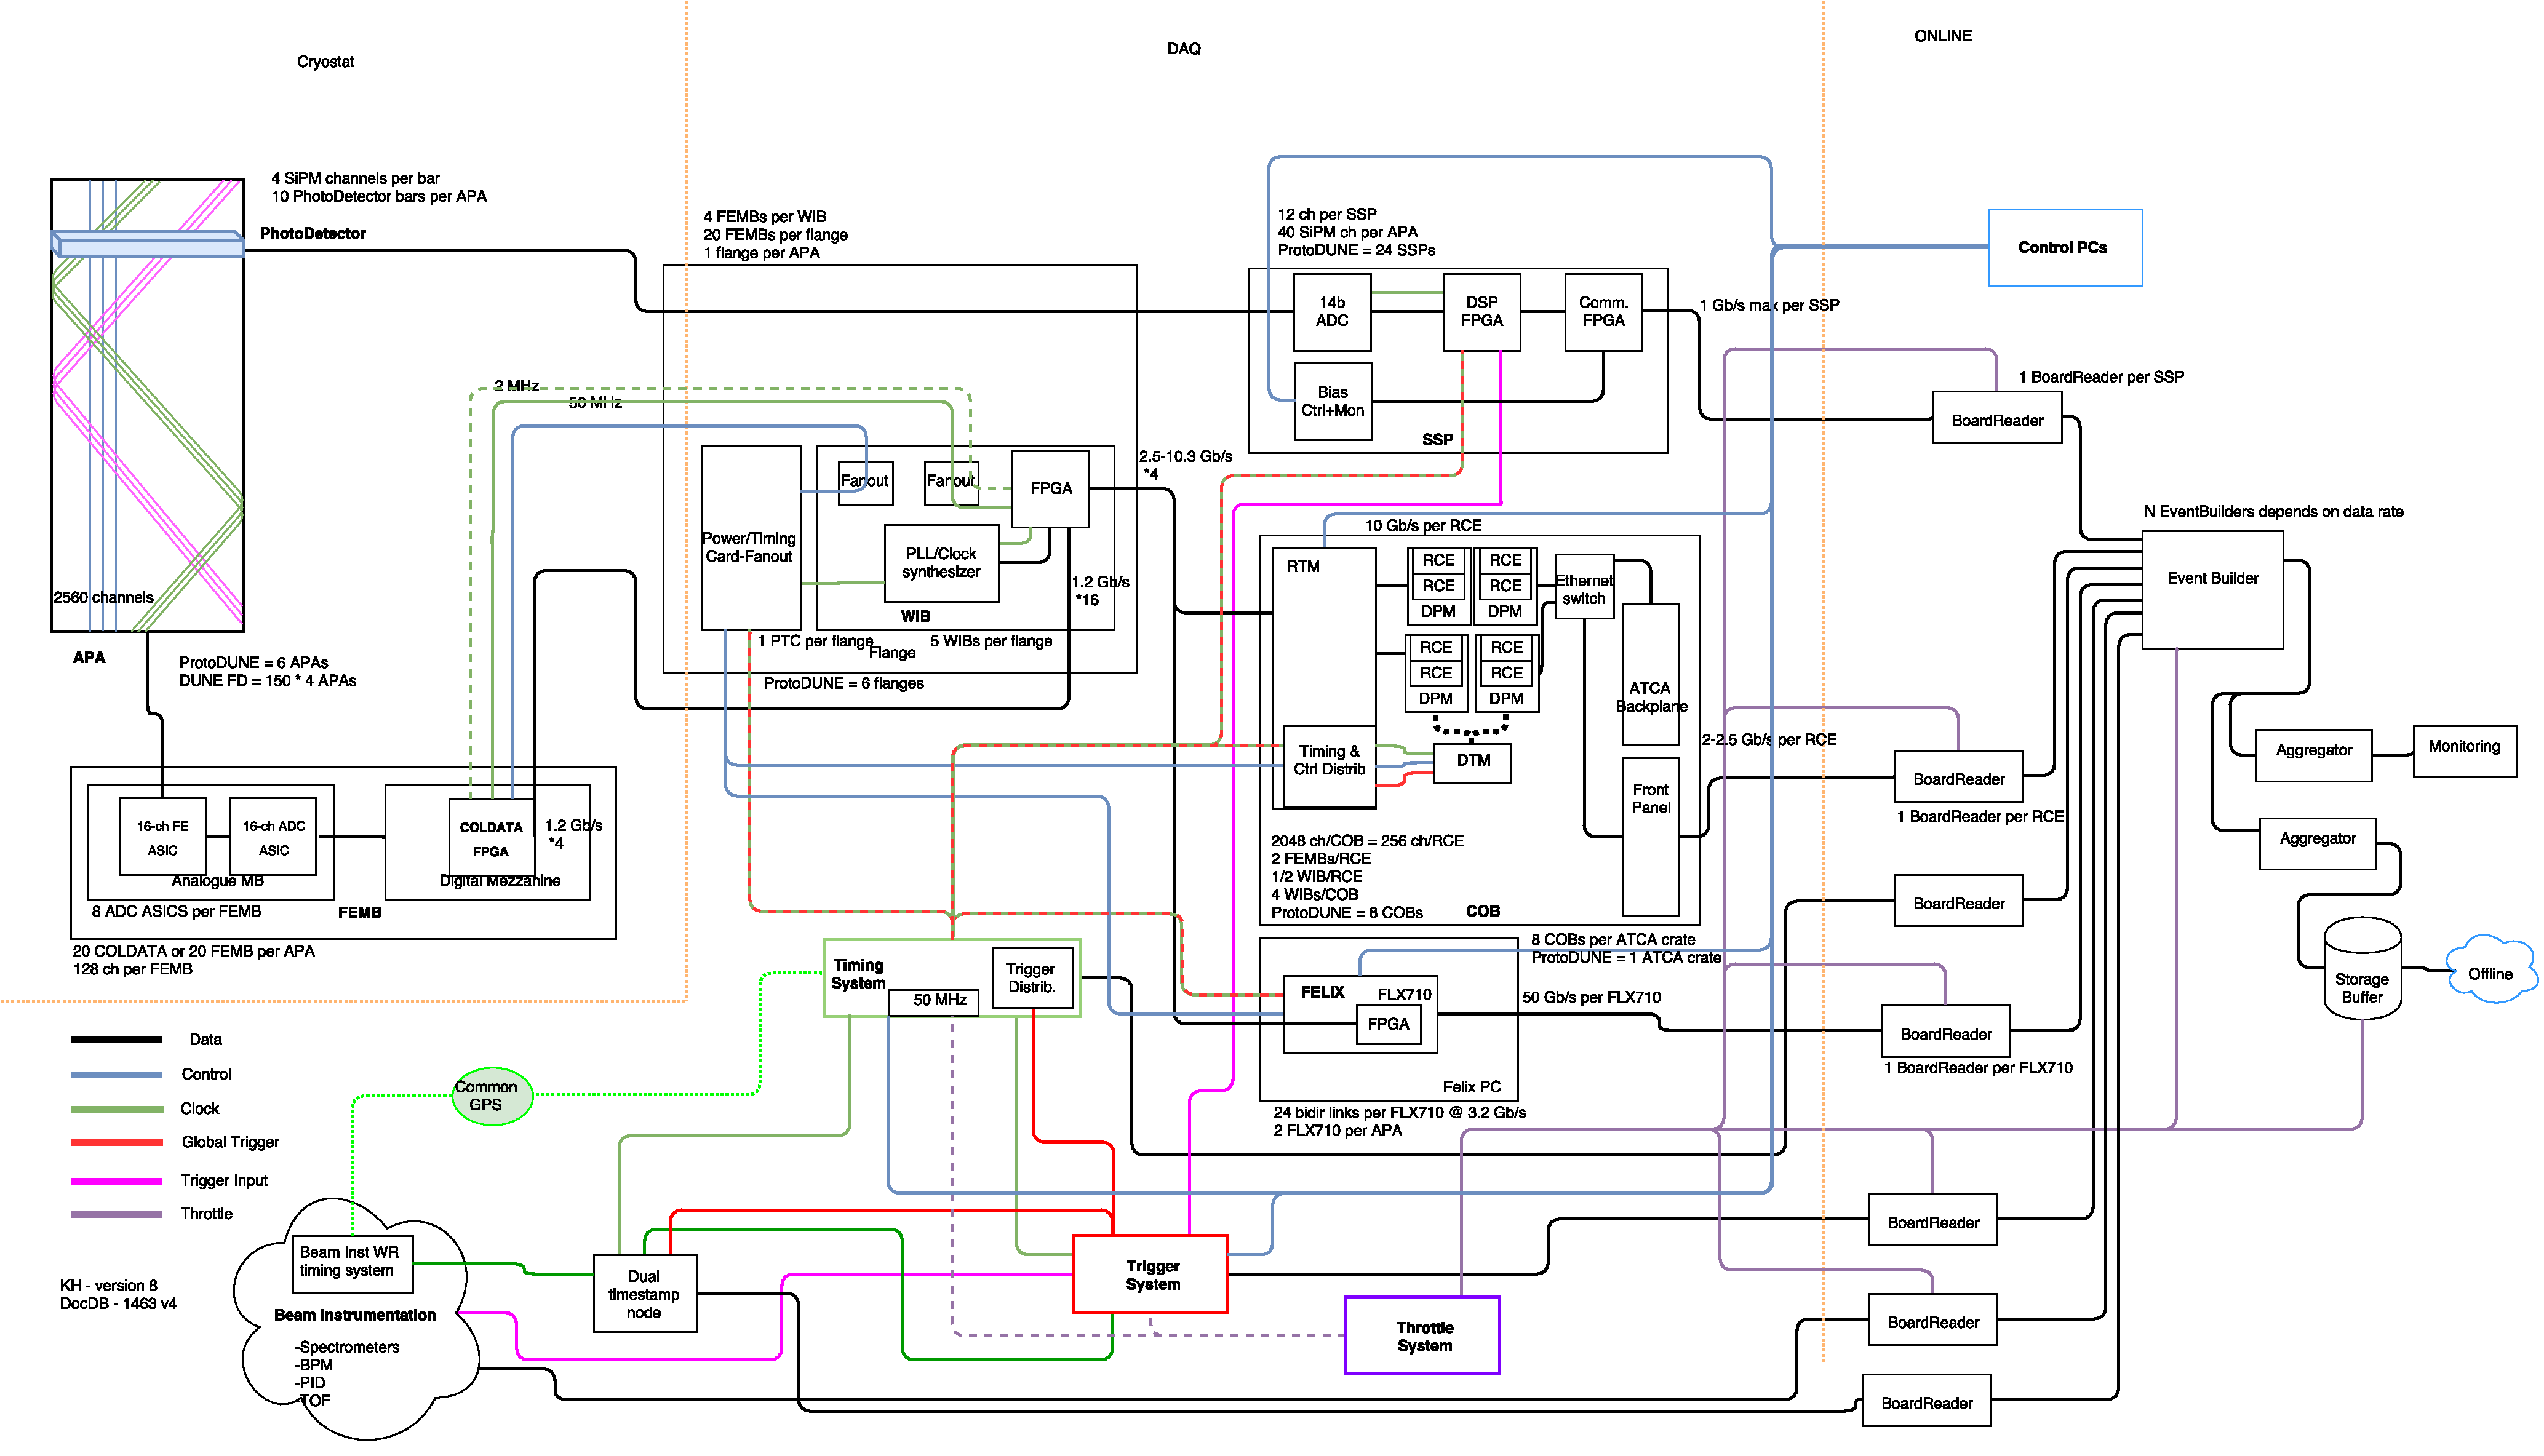
\includegraphics[angle=90,width=0.70\textwidth]{daq-overview-dia.pdf}
\end{cdrfigure}

%%%%%%%%%%%%%%%%%%%%%%%%%%%%%%%%%%%%%%%%%%%%%%
\subsection{TPC data reduction and collection}

Present the RCE system - just the main data flow, merging, compression etc.  State that the way the data ae collectd together, timing system, control etc., will be handled in section~\ref{sec:daq}, sentence at the end to say that the architecture allows future readout schemes to be incorporated and tested with ProtoDUNE and that these will be discussed, in particular the FELIX system, in subsection~\ref{ssec:daqfelix} 

%%%%%%%%%%%%%%%%%%%%%%%%%%%%%%%%%%%%%%%%%%%%%%
\subsection{PDS data reduction and collection}



%%%%%%%%%%%%%%%%%%%%%%%%%%%%%%%%%%%%%%%%%%%%%%

%%%%%%%%%%%%%%%%%%%%%%%%%%%%%%%%%%%%%%%%%%%%%%
\subsection{Introduction}

Brief overview of requirements for the collection of data for the primary goals.  (what subdetectors exist (TPC, PDS, trigger, beam counter monitoring, is there a beam position monitor (wire chamber or fiber detetor in the beam), a cosmic veto, a beam halo veto?  If so, who is doing these things?), primary readout scheme, alternative readout schemes including FELIX (section~\ref{ssec:daqfelix}) what the data rates are for the beam, need for calibration etc.).  Description of modes of operation (triggered, extended test modes for far detector).

Overview of how the DAQ will be commissioned (importance of online monitor early (and therefore need early definition of data format and simulation). 

Diagram: Physical connections between the main modules, showing the RCEs, FELIX, SSPs, and some generic beam detector readout.  Show timing system and show exiting arrows for where data are feeding the slow control.  Have the offline as a generic blob (i.e. details of data distribution are in a different section)

Descrine the above diagram.  Give table of rates in each branch, and make the comments on the data rates (i.e. anticipate questions the reviewers may have about bottlenecks).

%%%%%%%%%%%%%%%%%%%%%%%%%%%%%%%%%%%%%%%%%%%%%%
\subsection{Timing and trigger distribution}

Describe timing.  Paragraph giving requirements (point out where capabilities are better).  Possibly diagram showing WIB-RCE-timing.  Description of WIB-RCE interaction.  Also small paragraph about trigger logic - e.g. look at what LArIAT - I think it is a CAEN module, (Mike Kordosky at W\&M)

%%%%%%%%%%%%%%%%%%%%%%%%%%%%%%%%%%%%%%%%%%%%%%
\subsection{Event building software and DAQ computing farm }

Describe artDAQ, data handling caapbabilities, current plans, extensions forseen for final DUNE, throughput tests already made and planned.  Control of artDAQ processes (DAQIFACE), error handling, debugging emulation mode.

%%%%%%%%%%%%%%%%%%%%%%%%%%%%%%%%%%%%%%%%%%%%%%
\subsection{Slow control}

Description of scope (i.e. not beam, not cryo-system detectors.  Contains cryo-extra detectors (i.e. extras independent of needs of cryogenics systems).  Contains power off/on of equipment, monitoring of aTCA crates, SSP-voltages etc, DAQ rates etc.   Description of system chosen.  Listings of interfaces (in particular where a common Ethernet port is used for slow conrol and run control, such as on the WIB or SSP). 

%%%%%%%%%%%%%%%%%%%%%%%%%%%%%%%%%%%%%%%%%%%%%%
\subsection{User control interface}

(a.k.a. run control) [Before writing, it would be good to clarify the relationship between the two options (1) Erik Blaufuss's ICECUBE philosophy to put all run conrol into one browser interface with one authentication point, which is excellent and (2) either CERN WIN-xx or EPICS/CAA uBooNE system which are off the shelf environments.   How to decide - want biggest team of people with >30%fTE + commitment to be at CERN for ~3months over next 2 years, and then let them decide]]

%%%%%%%%%%%%%%%%%%%%%%%%%%%%%%%%%%%%%%%%%%%%%%
\subsubsection{Alternative readouts - FELIX}
\label{ssec:daqfelix}

Short paragraph saying that alternative readouts can be tested by replacing or adapting the WIBs to feed new systems.  A particular development which we want to persue vigerously is the FELIX system developed by a consortium incluing CERN, BNL, NIKHEF for ATLAS and for which all of these groups and PNNL are persuing for DUNE.   However, it is not a requirement that this readout is operating on day 1 of ProtoDUNE.

%%%%%%%%%%%%%%%%%%%%%%%%%%%%%%%%%%%%%%%%%%%%%%
\subsubsection{Other detector readout}

When groups are known, describe how integration of beam counter monitoring, beam position monitors (wire chambers of fibre detectors in the beam to measure position and improve momentum resolution) will be done. also cosmic veto or halo veto around beam.   For the beam counter monitoring, it may be that the 35t Penn trigger board could be used.

%%%%%%%%%%%%%%%%%%%%%%%%%%%%%%%%%%%%%%%%%%%%%%
\subsection{Software filtering and data transfer to permanent storage}

Point out that compression and/or further event sorting can be done in either the artDAQ trigger farm, or the online computng farm (run by the S\&C group).  Describe where we are on this (i.e. what compression algorithms, etc.  experience from other experiments).  Describe how the handoff to the S\&C processes writing to permanent storage work. Address the question of disk writing speeds.


